\documentclass[11pt]{article}
\usepackage[utf8]{inputenc} % allow utf-8 input
\usepackage[T1]{fontenc}    % use 8-bit T1 fonts
\usepackage[autonum,tchypersetup]{tchdr}
\usepackage{enumerate}
\usepackage[sort&compress]{natbib} % citep/citet
\usepackage{fancyhdr}
\usepackage{jmlr2e} % jmlr style file
\usepackage{float}


\newcommand{\distChiSq}{\chi^2}
\newcommand{\ltri}{\mathrm{tril}\,}
\newcommand{\block}{\mathrm{blockd}\,}


% Heading arguments are {volume}{year}{pages}{submitted}{published}{author-full-names}


% Short headings should be running head and authors last names
% \ShortHeadings{Learning with Mixtures of Trees}{Meil\u{a} and Jordan}
\firstpageno{1}

\begin{document}

\title{Computational discussion on robust variable selection via exponential square loss}

\author{\name Zuheng(David) Xu \email zuheng.xu@stat.ubc.ca \\
       \addr Student number: 24617185\\}      

% \editor{Leslie Pack Kaelbling}

\maketitle



%%%%%%%%%%%%%%%%%%%%%%%%%%%%%%%%%%%%%%%%%%%%%%%%%%%%%%%%%%%%%%%%%%%%%%%%
%% Main body of the paper
%% including sections 
%%%%%%%%%%%%%%%%%%%%%%%%%%%%%%%%%%%%%%%%%%%%%%%%%%%%%%%%%%%%%%%%%%%%%%%%
\section{Introduction} \label{sec:intro}
Robust variable selection problem has  gain much attention currently as it enables the identification of certain features and maintains resistance to outliers. A general framework is to consider a penalized regression problem with some robust loss function applied. The statistical property and computational feasibility of such problem highly depends on the loss itself and the penalty term. Usually, the loss function encodes the robustness and the penalty term enables the variable selection. 


With the goal of designing a robust estimator with high efficiency and maintaining optimal breakdown point, \citet{wang2013robust} proposes the exponential square loss function regularized by an adaptive LASSO penalty term, named ESL-LASSO method. 
In this report, we provide a complete introduction of the ESL-LASSO method with the focus on its computation. The code that implements the method and conduct empirical experiments is documented in \url{https://github.com/zuhengxu/qua4}.


In general this is a theory-oriented methodology, of which the design---specifically the procedure of choosing tuning parameters---is completely motivated by achieving the oracle property \citep{fan2001variable} and an optimal  asymptotic breakdown point. Although mathematically appealing,  the authors do not take careful treatments in the computational aspect, making the proposed method less practical and not reliable in many scenarios. Later in \cref{sec:computation}, we will discuss the limitation of the proposed method and point out potential challenges that occur in implementation. 



To resolve these problems, we present a simple iterative optimization scheme to solve the ESL-LASSO objective, as well as introducing a new tuning parameter selection procedure, yielding a significant improvement over the original ESL-LASSO method. 
The detailed presentation of our methods is provided in \cref{sec:computation}.
Finally, we compare the modified ESL-LASSO method with PENSE-LASSO \citep{freue2019robust} on three synthetic examples. The complete simulation results is included in \cref{sec:sim}.

\section{Robust variable selection} 
The key problem that \citet{wang2013robust} try to investigate is the  characterization of robustness when combining a variable selection process to a robust regression problem. Mathematically, the regression problem is formulated as a  minimization of some penalized robust loss function, where the robustness comes from a proper choice of the loss function and the sparsity of the solution is encoded in the penalty term. In this section, we introduce the penalized robust regression objective function and set up the notation for this report.


\subsection{Exponential square loss function} \label{sec:esl}
In the setting of robust regression, we are given a set of data points $\{(x_i, y_i)_{i=1}^n: \forall i\in [d],  x_i \in \reals^d, y_i \in \reals\}$, where $x_i$ is referred as the covariates and $y_i$ is the response. Assuming that $(x_i, y_i)$ satisfying the linear regression model:
\[
y_i = x_i^T \beta +\eps_i, \quad \forall i = 1, 2, \dots , n,     
\] 
and the goal is to infer the coefficients $\beta \in \reals^d$. 

The authors consider the exponential square loss (ESL) function with a tuning parameter $\gamma$, i.e., $\phi_\gamma(t)= 1-  \exp (-t^2/\gamma)$. And the unregularized empirical loss is given by
\[
 \ell_n^* = 1- \frac{1}{n}\sum_{i = 1}^ n \exp \left\{ -(y_i- x_i^T\beta)^2/\gamma\right\}  .    
\]
As illustrated in \cref{fig:esl}(Left), in contrast to the traditional OLS loss, the boundedness of this loss function limits the influence of outliers that generates huge residual error and controls the bias of the estimator. And the  
parameter $\gamma$ controls the level of the robustness by setting different ``truncation level'' to large residuals---as displayed in \cref{fig:esl}(Right), 
smaller $\gamma$ leads to a more robust estimator; on the other hand, it may increase the variance of the estimator as it focuses on data points that generate small residual errors.  

One may notice that ESL loss is not convex, meaning that solving the regression problem requires a careful choice of the initial value and optimization algorithm.
A comprehensive discussion of the optimization algorithm will be presented in \cref{sec:computation}.




\begin{figure}[H]
    \centering
    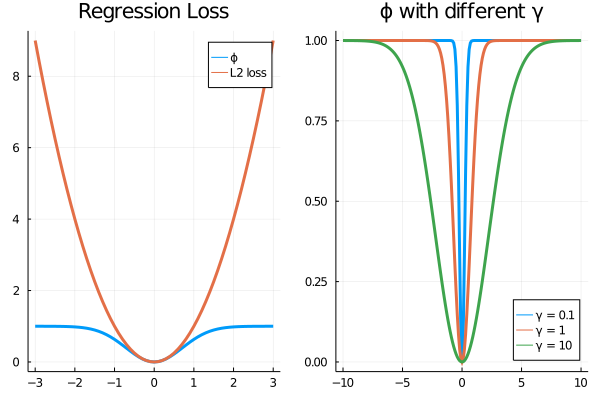
\includegraphics[width = 0.8\linewidth]{figures/esl.png}
    \caption{Figure of ESL loss function.}
    \label{fig:esl}
\end{figure}






\subsection{Regularizer} \label{sec:pnty}
Next, we introduce the regularization term that encodes the sparsity to the estimator, namely enables a variable selection. A typical choice is the $\ell_1$ penalization, i.e., $\|\beta\|_1$, which is widely used in a linear regression setting (LASSO). However, researchers find that the LASSO is not consistent in general, meaning that it may not recover the true underlying model asymptotically \citep{zhao2006model}. Therefore, \citet{wang2013robust} propose using the adaptive LASSO penalty \citep{zou2006adaptive} with tuning parameters $\tau_{nj}$, 
\[
p_{\tau}(\beta) = \sum_{j=1}^d \tau_{nj}|\beta_j|/|\tilde{\beta_j}|,   
\]
which can be viewed as a weighted version of $\ell_1$ norm.
Here $\tilde{\beta}$ is an pilot robust regression estimator, e.g., MM-estimator, S-estimator, OLS estimator, which should be chosen as a $\sqrt{n}$-consistent estimator. As suggested by the authors, we set $\tilde \beta$ as the MM-estimator, which later is also used as the initial value of the optimization algorithm. 


Intuitively, the regularizing constant $\tau \defined (\tau_{n1}, \dots, \tau_{nd}) $ controls the level of this weighted $\ell_1$ penalization, i.e., $\sum_{j = 1}^d \frac{\tau_{nj}}{|\tilde{\beta_j}|} |\beta_j|$. For a fixed pilot estimator $\tilde{\beta}$, larger value of $\tau$ tends to return a sparser estimator.  
The author suggest simply setting 
\[
 \tau_{n1} = \dots = \tau_{nd} = \frac{\log n}{n} =: \tau_n,
\] 
which comes from the minimization of a BIC-type objective function. Therefore, the ESL-LASSO estimator is defined as the minimizer of the following objective function:
\[\label{eq:esl_lasso}
\ell_n(\beta)  =    1- \frac{1}{n}\sum_{i = 1}^ n \exp \left\{ -(y_i- x_i^T\beta)^2/\gamma\right\} +  \tau_{n} \sum_{j=1}^d|\beta_j|/|\tilde{\beta_j}|.
\]
The goal of using this combination of $\tau_n$ and the adaptive LASSO penalty is to ensure a stronger asymptotic property for the ESL-LASSO estimator in terms of the variable selection process, which is called the \emph{oracle property} \citep{fan2001variable}---not only identifies the true coefficients in data asymptotic regime, but also obtains the optimal convergence rate. 























\section{Computation}\label{sec:computation} Given the non-convexity of the
loss function, the non-smooth $\ell_1$
penalty and two tunning constants, obtaining an efficient computation strategy that maintains the ideal statistical
properties is not trivial. The goal of this section is to provide an extensive discussion on the original
computational scheme, including the numerical algorithm and the way of making a reasonable choice on the tuning
parameters. Also, we present a few alternatives based on the our discussion on the original methods and provide a
detailed justification.


\subsection{Proximal gradient method} 

As the objective function \cref{eq:esl_lasso} is composited with both a
non-convex (ESL loss) and a non-smooth ($\ell_1$ regularizer) term, solving the optimization globally is difficult.
In the paper, for the feasibility of computation, the authors consider a global quadratic approximation to the loss
function at the initial estimator $\tilde{\beta}$ (MM-estimator as suggested by the author) , namely the actual
target function is as follows, 
\[\label{eq:quadrelax} \tilde{\ell}_n(\beta) = \frac{1}{2} (\beta - \tilde{\beta})^T
\nabla^2 \ell_n^*(\tilde{\beta}) (\beta - \tilde{\beta}) + \tau_n \sum_{j = 1}^d \frac{|\beta_j|}{|\tilde{\beta_j}|}. \] 
Recall that $\ell^*_n(\beta) = 1 -\frac{1}{n}\sum_{i = 1}^ n \exp \left\{ -(y_i-
x_i^T\beta)^2/\gamma\right\}$. Then there is a plenty of efficient algorithms can be used to solve this type of
problem, such as coordinate descent method \citep{wu2008coordinate}, the alternating direction method of multipliers
(ADMM) \citep{ouyang2013stochastic} and etc, among which \citep{wang2013robust} pick the coordinate descent
algorithm.

Though this $\ell_2$ relaxation could enable a solvable optimization, there are some concerns with this idea. The
first minor issue is that the optima of \cref{eq:esl_lasso} do not coincide with \cref{eq:quadrelax}, meaning that we
have no guarantees on the solution of this relaxed problem. Second, the global minimum of \cref{eq:quadrelax} may not
exist. In fact, due to the non-convexity of $\ell_n^*(\beta)$, $\nabla^2 \ell_n^*(\tilde \beta)$ is not guaranteed to
be semi-positive definite, in which case \cref{eq:quadrelax} is not even lower bounded. \cref{fig:lstar} visualizes
the $\ell_n^*(\beta)$ under a $1$-dimensional simulated dataset under different value of $\gamma$, from which we can
clearly see the shape of $\ell_n^*$ depends on the dataset as well as the choice of $\gamma$.


\begin{figure}[t!] 
    \centering 
    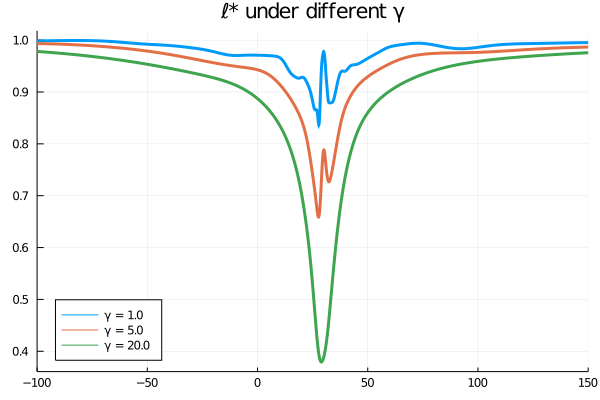
\includegraphics[width = 0.8\linewidth]{figures/lstar.png}
     \caption{Figure of $\ell_n^*$ on a synthetic dataset.} \label{fig:lstar} 
\end{figure}


Further, assuming the optimum of \cref{eq:quadrelax} is well defined, there is a fundamental flaw of this global
convex relaxation strategy---$\ell_2$ loss is not a robust loss function. To limit the influence of outliers, the
loss function of a robust regression is usually bounded above (meaning that it has to be non-convex), then the the
outliers cannot bias the estimates arbitrarily. A good example is the proposed ESL loss function $\phi_\gamma$.
However, replacing the ESL loss with a quadratic function completely ruins the robustness and could lead to a
non-sense estimates when the dataset is contaminated. The only situation where such quadratic approximation is
acceptable is that when the initial estimator $\tilde{\beta}$ smartly picked such that it lies in a local convex
region around the true optimum $x^*$, i.e., 
\[ 
    \tilde \beta \in \{ \mcB_\delta(x^*): \delta >0 \text{ and }\ell_n(\beta) \text{ is convex inside } \mcB_\delta(x^*)\}. 
\] 
Then there is some hope that the true solution can be
recovered by optimizing on this quadratic surrogate objective.

Therefore, to address these issues, we propose a new algorithm---\emph{proximal gradient descent method} (proximal
GD)---of solving \cref{eq:esl_lasso}, which is a simple iterative algorithm. Before the presentation of the detailed
implementation of proximal GD, we provide a brief introduction to the general proximal gradient method
\citep{parikh2014proximal}. Proximal gradient method is commonly applied to the optimization problem with non-smooth
regularizer, e.g., LASSO, elastic net, compressed sensing. Considering the general optimization problem as follows,
\[ \min_{x \in \reals^d} f(x) + g(x), \] where $f$ is differentiable; and $g$ is convex but not necessarily
differentiable. In the ESL-LASSO problem setting, $f$ is the ESL empirical loss function $ \ell_n^*$ and $g$ is the
adaptive lasso penalty. The iteration of proximal gradient method is given as follows, \[\label{eq:proxiter} x_{k+1}
&= \prox{\alpha_k, g}{x_k - \alpha_k \nabla f(x_k)}, \quad k\in \nats. \] where $\alpha_k > 0 $ is the step size at
each iteration and $\prox{\alpha_k, g}{\cdot}$ is the proximal operator. Specifically, let $x_k' = x_k - \alpha_k
\nabla f(x_k)$, \cref{eq:proxiter} can be written into: \[ x_{k+1} &= \prox{\alpha_k,g}{x_k'} = \argmin_{z\in
\reals^d} \frac{1}{2\alpha_k} \|z - x_k'\|_2^2 + g(z). \] Interestingly, the proximal gradient method can be
interpreted as a particular case of the \emph{majorization-minimization algorithm} (MM algorithm), a wide class of
algorithms that are popular for non-convex optimization. The key of the MM algorithm is by minimizing a tight convex
upper bound of the original objective function and decreasing the object value after each iteration. The most well
known example of the MM algorithm in statistical literature is the EM algorithm. Suppose $f$ is $L$-smooth---if $f$
is twicely continuous differentiable, $\nabla^2 f \preceq LI, L> 0 $. Then an upper bound of $(f+ g) (x)$ can be
given by \[ f(y) + \nabla f(y)^T(x- y ) + \frac{1}{2 \alpha} \| x- y\|_2^2 +g(x), \quad \alpha \in (0, L^{-1} ], \]
which is convex on $x$ for a fixed $y$ and touches the original function $f + g$ as $x = y$. Substituting $y = x_k,
\alpha = \alpha_k$ and minimizing over $x$ precisely gives the proximal GD iteration \cref{eq:proxiter}, as long as
the step size $\alpha_k$ is carefully chosen.

Therefore, applying the scheme of proximal gradient method to the ESL-LASSO problem yields the following numerical
iteration: \[\label{eq:eslproxiter} \beta_{k+1} \gets \text{Prox}_{\alpha_k, \mathcal{P}}(\beta_k - \alpha_k \nabla
\ell_n^*(\beta_k)), \quad \alpha_k \leq \left(\frac{2}{\gamma} \sigma_1\left(\frac{1}{n} \sum_{i=1}^n x_i x_i^T
\right)\right)^{-1}, \] where $ \text{Prox}_{\alpha_k, \mathcal{P}}(\cdot)$ is the proximal operator and
$\mathcal{P}(\beta) = \sum_{j = 1}^d \frac{\tau_{nj}}{|\tilde{\beta_j}|} |\beta_j|$; and $\sigma_1(M )$ denotes the
maximal singular value of matrix $ M$. The following proposition provides a simple upper bound on the Lipschitz
constant of $\ell_n^*$. \bnprop For all $\beta \in \reals^d$, $\nabla^2 \ell_n^* (\beta) \preceq \frac{2}{\gamma}
\sigma_1\left(\frac{1}{n} \sum_{i=1}^n x_i x_i^T \right)$. \enprop \bprf

Write $ \ell_{(i)}^*(\beta) = 1- \exp \left\{ -(y_i- x_i^T\beta)^2/\gamma\right\}$ and hence $\ell_n^* =
\frac{1}{n}\sum_{i=1}^n \ell_{(i)}^*$. We can examine the gradient and Hessian of $\ell_{(i)}^*$ as follows: \[
\begin{aligned} \nabla^2 \ell_i^*(\beta) & = \frac{2}{\gamma} \left[ \exp\left(-\frac{2 r_i(\beta)^2}{\gamma} \right)
\left(1- \frac{2 r_i(\beta)^2}{\gamma} \right)\right] (x_i x_i^T) \\ & \preceq \frac{2}{\gamma} (x_i x_i^T),
\end{aligned} \] where $r_i(\beta)\defined x_i^T\beta - y_i$. This completes the proof. \eprf


\begin{algorithm}[t!] \caption{Proximal gradient descent} \label{alg:proxGD} \begin{algorithmic}
\Procedure{ProxGD}{$\beta_0$, $\gamma$ ,$(\alpha_k)_{k\in\nats}$, $(x_i)_{i=1}^n$} \State $\text{Compute Lipschitz
constant } L \gets \left(\frac{2}{\gamma} \sigma_1\left(\frac{1}{n} \sum_{i=1}^n x_i x_i^T \right)\right)^{-1}$
\For{$k=0, 1, \dots, K-1$} \State $\alpha_k \gets \min \left(\alpha_k ,L\right)$ \State $\beta_{k+1} \gets
\text{Prox}_{\alpha_k, \mathcal{P}}(\beta_k - \alpha_k \nabla \ell_n^*(\beta_k))$ (\cref{eq:ista}) \EndFor \State
\Return $\beta_K$ \EndProcedure \end{algorithmic} \end{algorithm}

This majorization-minimization nature of \cref{eq:eslproxiter} ensures producing iterates that converges to a local
optimum \citep{hunter2004tutorial}, but we have to mention that there is no theoretical guarantee that it will solve
the optimization globally. Another major reason for us to choose the proximal GD is that it is simple for
implementation, where the proximal operator has close form solution. For $\ell_1$ penalty, the proximal operator can
be written as the soft-thresholding operator: Let $\beta^+_k := \beta_k - \alpha_k \nabla \ell_n^*(\beta_k) $,
$\lambda_j = \frac{\tau_{nj}}{|\tilde{\beta_j}|}$. Then for $i=1, \ldots, d $, \[ \label{eq:ista}
\left[\text{Prox}_{\alpha_k, \mathcal{P}} (\beta^+_k) \right]_j= \left[S_{\lambda_j\alpha_k
}(\beta^+_k)\right]_{j}=\left\{\begin{array}{ll} \left[ \beta^+_k\right]_j-\lambda_j\alpha_k & \text { if } \left[
\beta^+_k\right]_j>\lambda_j \alpha_k \\ 0 & \text { if }-\lambda_j\alpha_k \leq \left[ \beta^+_k\right]_j \leq
\lambda_j\alpha_k \\ \left[ \beta^+_k\right]_j+\lambda_j\alpha_k & \text { if } \left[ \beta^+_k\right]_j<-\lambda_j
\alpha_k \end{array}\right. . \] The detailed implementation of this algorithm is presented in \cref{alg:proxGD}.


\subsection{Tuning parameter selection: the choice of $\gamma$}

To implement the methodology properly, it is
necessary to make sensible choice of the tunning constants, including $\tau_{nj}$ in the adaptive LASSO penalty and
$\gamma$ in the loss function. In the original paper, selection procedures are motivated by asymptotic theory. In
this section, we discuss the selection methods proposed by the author and provide our alternatives that improve the
performance of ESL-LASSO. Since the choice of $\tau$ is specified in \cref{sec:pnty}, in this section, we pay
attention on the selection of $\gamma$.

As we briefly mentioned in \cref{sec:pnty}, the choice of $\gamma$ determines the level of robustness. In fact, based on our empirical finding, the quality of the ESL-LASSO estimator is very sensitive to the value of $\gamma$. Also, as shown in \cref{fig:lstar}, we see that the optimization landscape may be influenced by the value of $\gamma$. Those information hints an important fact that the selection method of $\gamma$ should be designed carefully. 



The paper under discussion proposes a data-dependent procedure that  learns the value of $\gamma$, which includes three steps:
\benum
\item[Step 1: ] Identifying the pseudo outliers based on large residual error. Let $r_i(\beta) = x_i^T \beta - y_i, i = 1, 2, \dots, n $. The pseudo outlier set $D_m$ is selected by
\[\label{eq:pseudo_outlier}
D_m = \{(x_i, y_i): |r_i(\tilde\beta )| \geq 2.5 S_n| \}, \quad S_n = 1.4826 \times \text{med}_i | r_i(\hat \beta - \text{med}_j(r_j(\tilde \beta))   )| .
\]  
Here $m$ denotes the number of data points of $D_m$ and we denote the cleaned dataset as $D_{n-m}$.

\item[Step 2:] Selecting $\gamma$ that minimizes the asymptotic variance of $\tilde \beta$ in the range that ensures an asymptotic breakdown point at $1/2$, which uses $D_{n-m}$. Specifically, $\gamma$ is obtained by minimizing the determinant of the asymptotic covariance matrix $\hat{V}(\gamma)=\left\{\hat{I}_{1}\left(\hat{\beta}_{n}\right)\right\}^{-1}
\tilde{\Sigma}_{2}\left\{\tilde{I}_{1}\left(\tilde{\beta}_{n}\right)\right\}^{-1}$ within the range $G$, where 
\[ \label{eq:G}
    G =
\left\{\gamma: \frac{2m}{n} + \frac{2}{n}\sum_{ i =m+ 1}^n \phi_\gamma(r_i(\tilde \beta_n))\leq 1\right\}, \] 
and 
 \[
\begin{aligned} 
    \tilde{I}_{1}\left(\tilde{\beta}_{n}\right) 
    &=\frac{2}{\gamma}\left\{\frac{1}{n} \sum_{i=1}^{n} \exp \left(-r_{i}^{2}\left(\tilde{\beta}_{n}\right) / \gamma\right)\left(\frac{2r_{i}^{2}\left(\tilde{\beta}_{n}\right)}{\gamma}-1\right)\right\}\left(\frac{1}{n} \sum_{i=1}^{n} {x}_{i} {x}_{i}^{T}\right) \\ \tilde{\Sigma}_{2} 
    &=\operatorname{cov}\left\{\exp
\left(-r_{1}^{2}\left(\tilde{\beta}_{n}\right) / \gamma\right) \frac{2
r_{1}\left(\tilde{\beta}_{n}\right)}{\gamma} {x}_{1}, \cdots, \exp
\left(-r_{n}^{2}\left(\tilde{\beta}_{n}\right) / \gamma\right) \frac{2
r_{n}\left(\tilde{\beta}_{n}\right)}{\gamma} {x}_{n}\right\} 
\end{aligned}.
\]

\item[Step 3:] Obtaining  $\hat \beta$ by optimizing \cref{eq:esl_lasso}. And set $\tilde \beta = \hat \beta$.
\eenum
Note that both Step 1 and 2 depend on the current value of the estimates $\tilde \beta$. Thus to make sure the value of $\hat \beta$ and $\gamma$ converges, the author suggest iterating Steps 1-3 until convergence. In the initial round, the author suggest using the MM-estimator.
The key step above is the Step 2, which is completely originated from the asymptotic results. By \citet[Theorem 2.]{wang2013robust}, $\gamma \in G$ is necessary for the optimal asymptotic breakdown point of the ESL-LASSO estimator; and by minimizing the asymptotically variance, we expect to find the value of $\gamma$ leading to a faster convergence rate of the eventual estimator. This procedure sounds intuitively reasonable but is actually not reliable from both practical and statistical perspective.

In practice, there is basically no efficient way of solving the constrained optimization problem described in Step 2 as there is no structure of the feasible set $G$ and the target function is a determinant of a complicated matrix. As a result, the authors consider using grid search to identify the set $G$ and the solution of $\gamma$.  Although it sounds like brutal force, provided that $\gamma$ is a univariate variable, it is acceptable.  This procedure is illustrated in \cref{fig:gamma}---we simply plot $\xi(\gamma)\defined \frac{2m}{n} + \frac{2}{n}\sum_{ i =m+ 1}^n \phi_\gamma(r_i(\tilde \beta_n))$ and $\log \det (\hat V (\gamma))$  against $\gamma$; and then search the optimal choice of $\gamma$ along these two curves.    The tricky part for the implementation is to determine the searching range, which is obviously problem specific. In practice, one  may want to try a few different ranges to see whether the result is satisfying. Another interesting problem we find in the empirical experiment is that repeating Step 1-3 does not leads to a convergence. In all our simulation settings (introduced in detail in next section), iterating Step 1-3 will just send $\gamma$ to an unreasonable value and hence leads to a useless estimator. This contradicts to the claim in the paper that the whole process converges quickly and only requires two repetitions. 



\begin{figure}[t!]
    \centering
    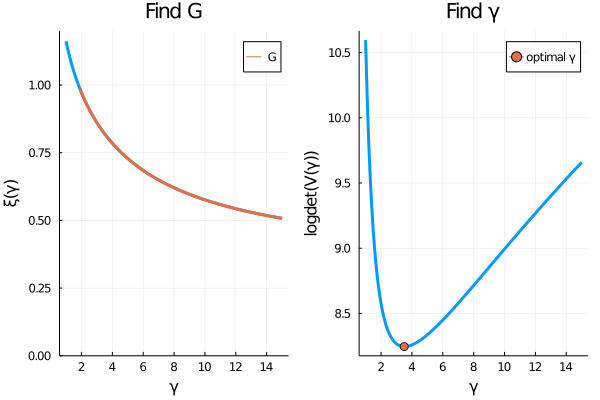
\includegraphics[width = 0.8\linewidth]{figures/gamma_plot.png}
    \caption{(Left) $\xi(\gamma)$ against $\gamma$; (Right) $\log \det (\hat V (\gamma)) $   against $\gamma$. The curves are based on the synthetic dataset with $n = 800$, $d = 8$ and true coefficients $\beta  =(1, 1.5, 2, 1, 0,0,0,0)^T$. $x_i\distiid \distNorm(0, \Omega)$, $[\Omega]_{i,j} = 0.5^{|i-j|}$. } \label{fig:gamma}
\end{figure}



However, this selection scheme on $\gamma$ represents a fundamental misunderstanding to the robust regression problem. A general rule of designing a robust estimator is to balance the robustness and
the efficiency of the estimator. In other words, we need to ensure a sensible bias-variance trade-off. The major
problem of focusing on choosing $\gamma$ that leads to minimal asymptotic variance is that it overlooks the bias and
could result in an non-robust estimator. We find out in the simulation that this procedure works fine without the
presence of outliers but is not reliable when the dataset is contaminated with outliers, which aligns with our
intuition above.
Specifically, in our empirical findings, Step 2 tends to search for an abnormally large $\gamma$, yielding a vacuous estimates $\hat \beta_n = (0,0, \dots ,0)^T $. 
 
To resolve these issues, we propose a new procedure of selecting a proper $\gamma$, which is generally simpler and more reliable comparing to the original procedure.   
We focus on the intuition that the $\gamma$ serves as a scale parameter that controls the importance of the residual error.
Therefore, a naive idea is to use the estimated residual variance. However, considering the presence of outliers, estimating the residual variance with the raw dataset may lead to a huge bias. Thus, a better choice is to combine with the Step 1 that discards the pseudo outliers from  the raw dataset and estimate the residual variance with ``cleaned'' dataset $D_{n - m}$, of which is updates of $\gamma$ is given by 
\[
    \gamma \gets \frac{1}{n-m} \sum_{i = m+1}^n ( y_i - x_i \beta )^2.
\]
Note that similar to the original method, this updates also depend on the current estimates of $\beta$. Thus, we may also want to iterate between the $\gamma$ selection and solving \cref{eq:esl_lasso} with proximal GD as proposed in the paper. The detailed implementation for the complete procedure of  ESL-LASSO estimation is then provided in \cref{alg:esl_lasso}. 

\begin{algorithm}[t!] 
    \caption{ESL-LASSO estimation} \label{alg:esl_lasso} 
\begin{algorithmic}
   \Procedure{ESL-LASSO}{$\tilde \beta$, $\gamma$ ,$(\alpha_k)_{k\in\nats}$, $(x_i)_{i=1}^n$} 
   \State $\tilde \beta \gets \text{MM-estimator}$
   \State $ k = 0$
   \For{ $k=0, 1, \dots, K-1$}
\State Identifying the pseudo outliers $D_m$ (\cref{eq:pseudo_outlier})
\State $\gamma \gets \frac{1}{n-m} \sum_{i = m+1}^n ( y_i - x_i \beta )^2$
\State $\hat \beta \gets \text{ ProxGD}(\tilde \beta$, $\gamma$ ,$(\alpha_k)_{k\in\nats}$, $(x_i)_{i=1}^n) $ (\cref{alg:proxGD})
\State $\tilde{ \beta }\gets \hat \beta, \quad k \gets k+1$ 
\EndFor
    \State \Return $\hat \beta$ 
   \EndProcedure 
\end{algorithmic}
\end{algorithm}





\section{Simulation} \label{sec:sim}



\begin{figure}[t]
    \centering
    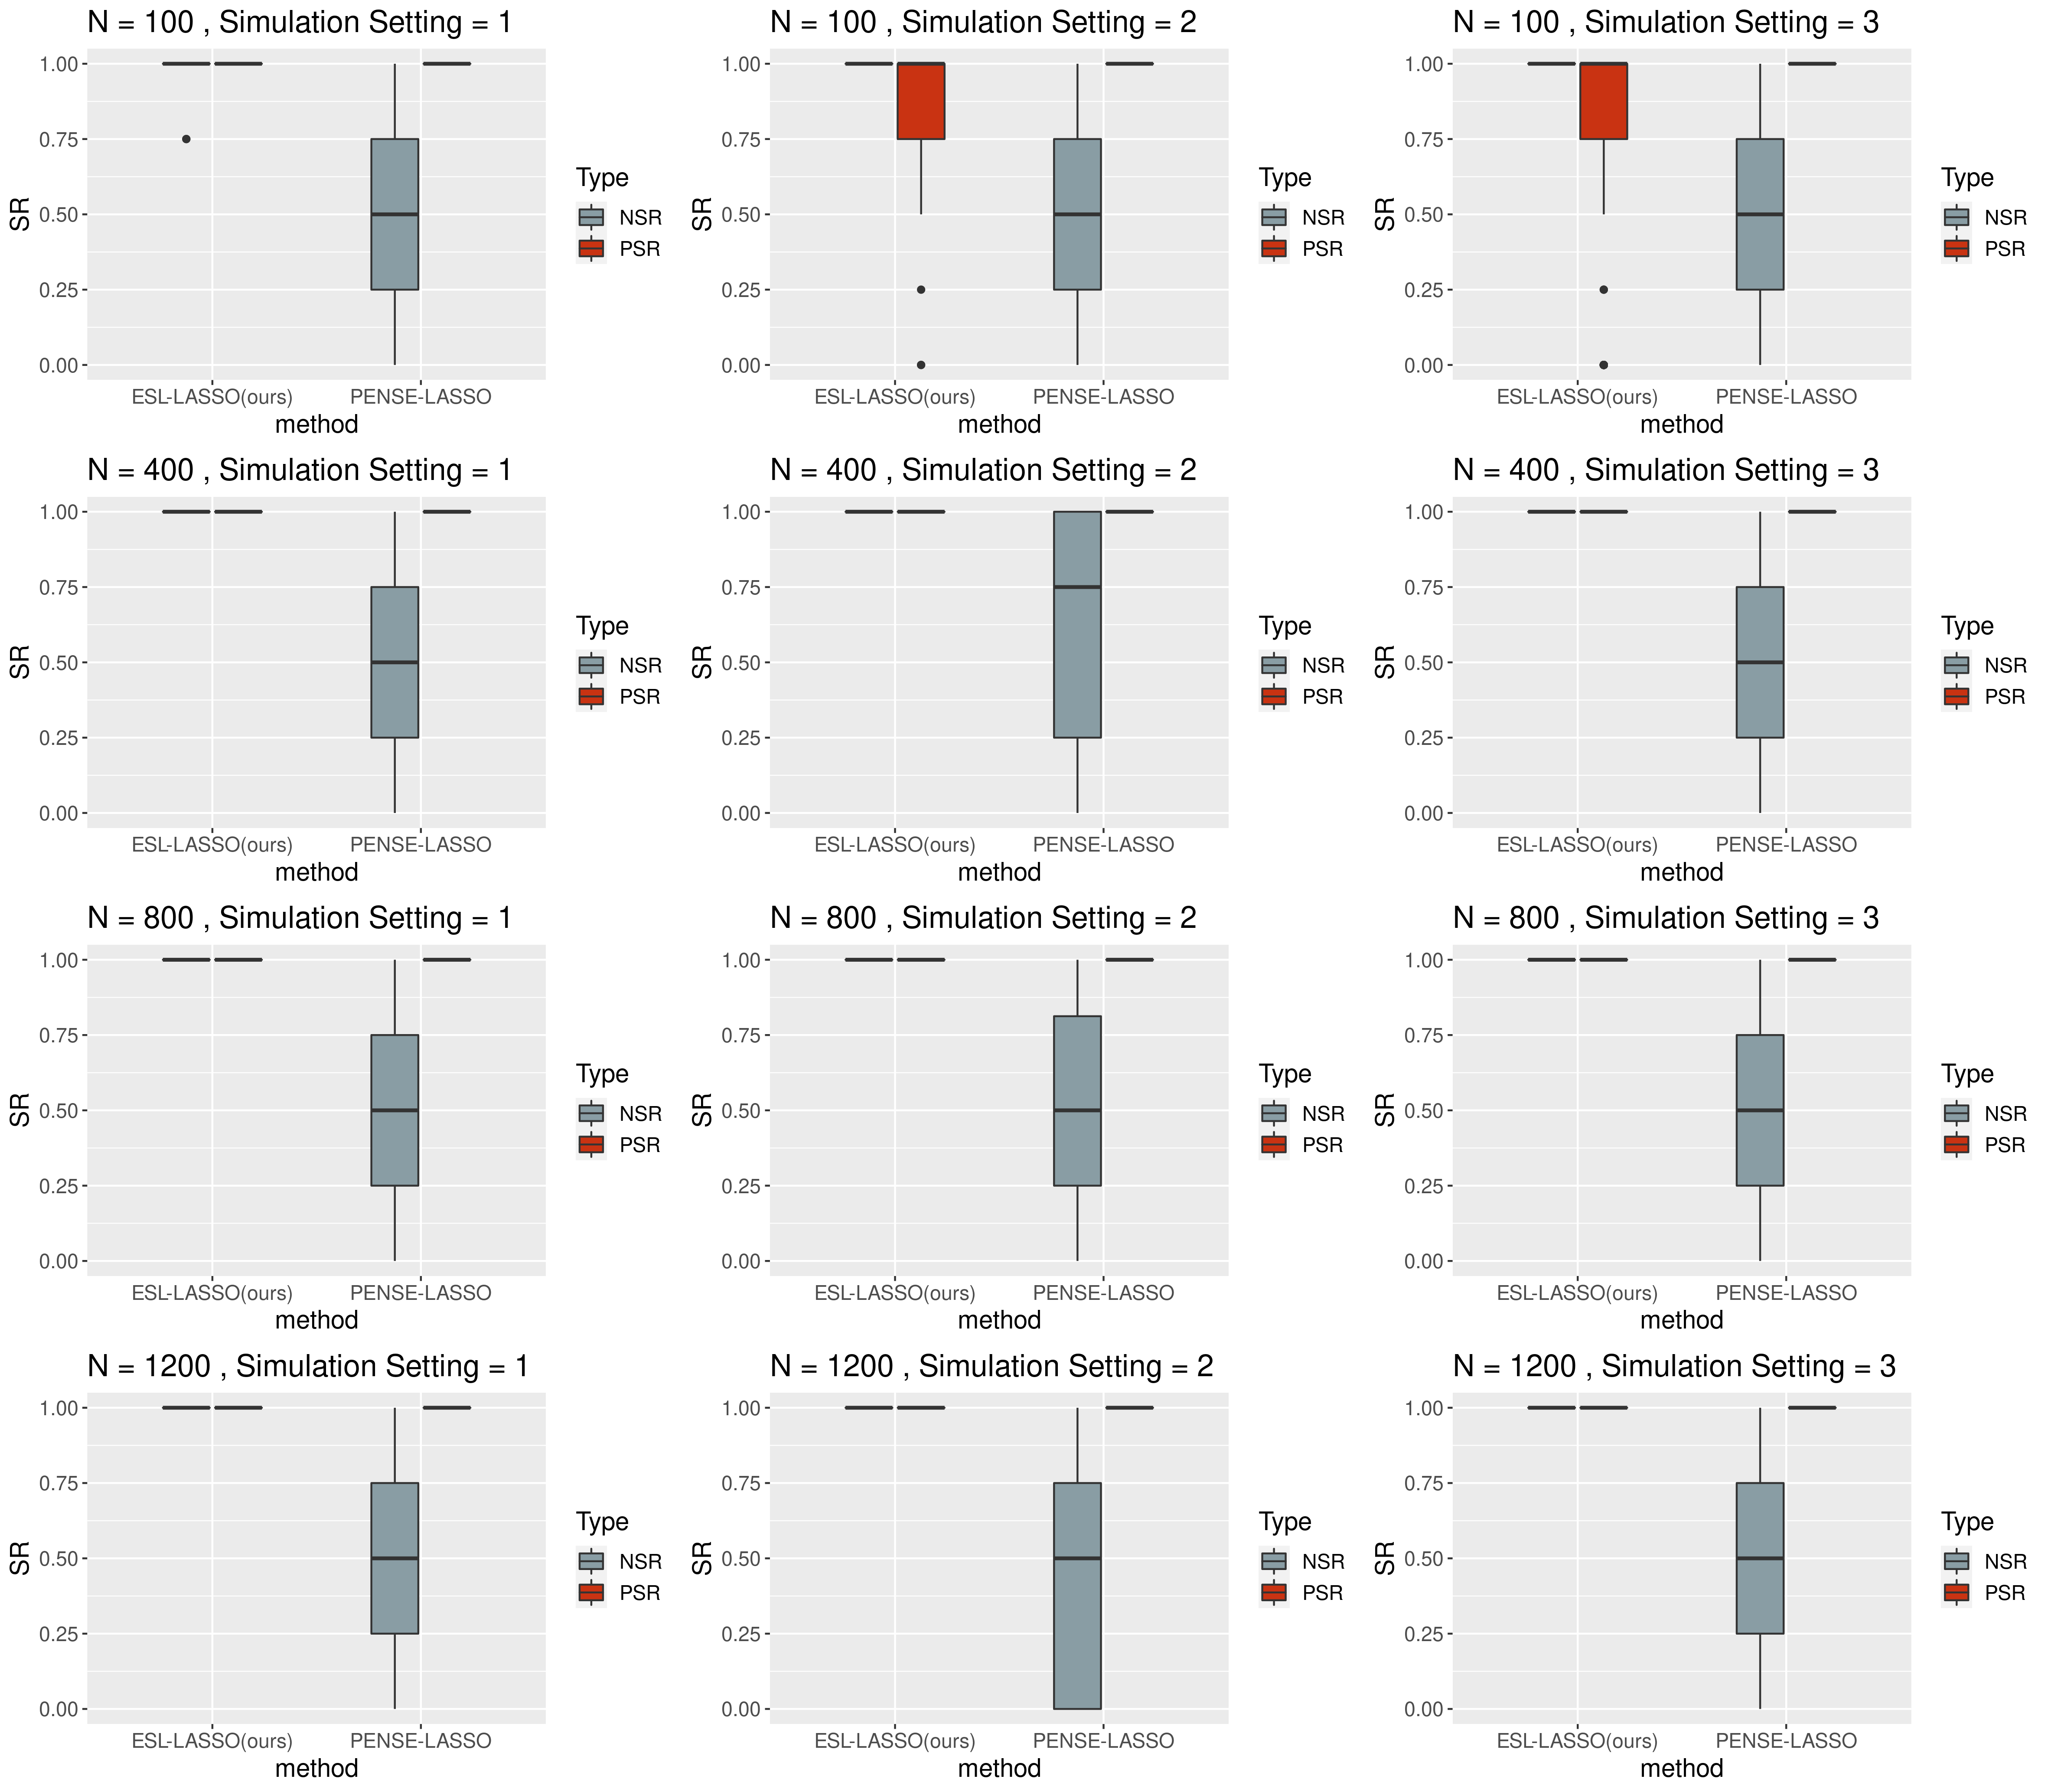
\includegraphics[width = \linewidth]{figures/SR_compare.png}
    \caption{Box plots for the variable selection rate across all simulation settings. }
    \label{fig:sr}
\end{figure}



\begin{figure}[t]
    \centering
    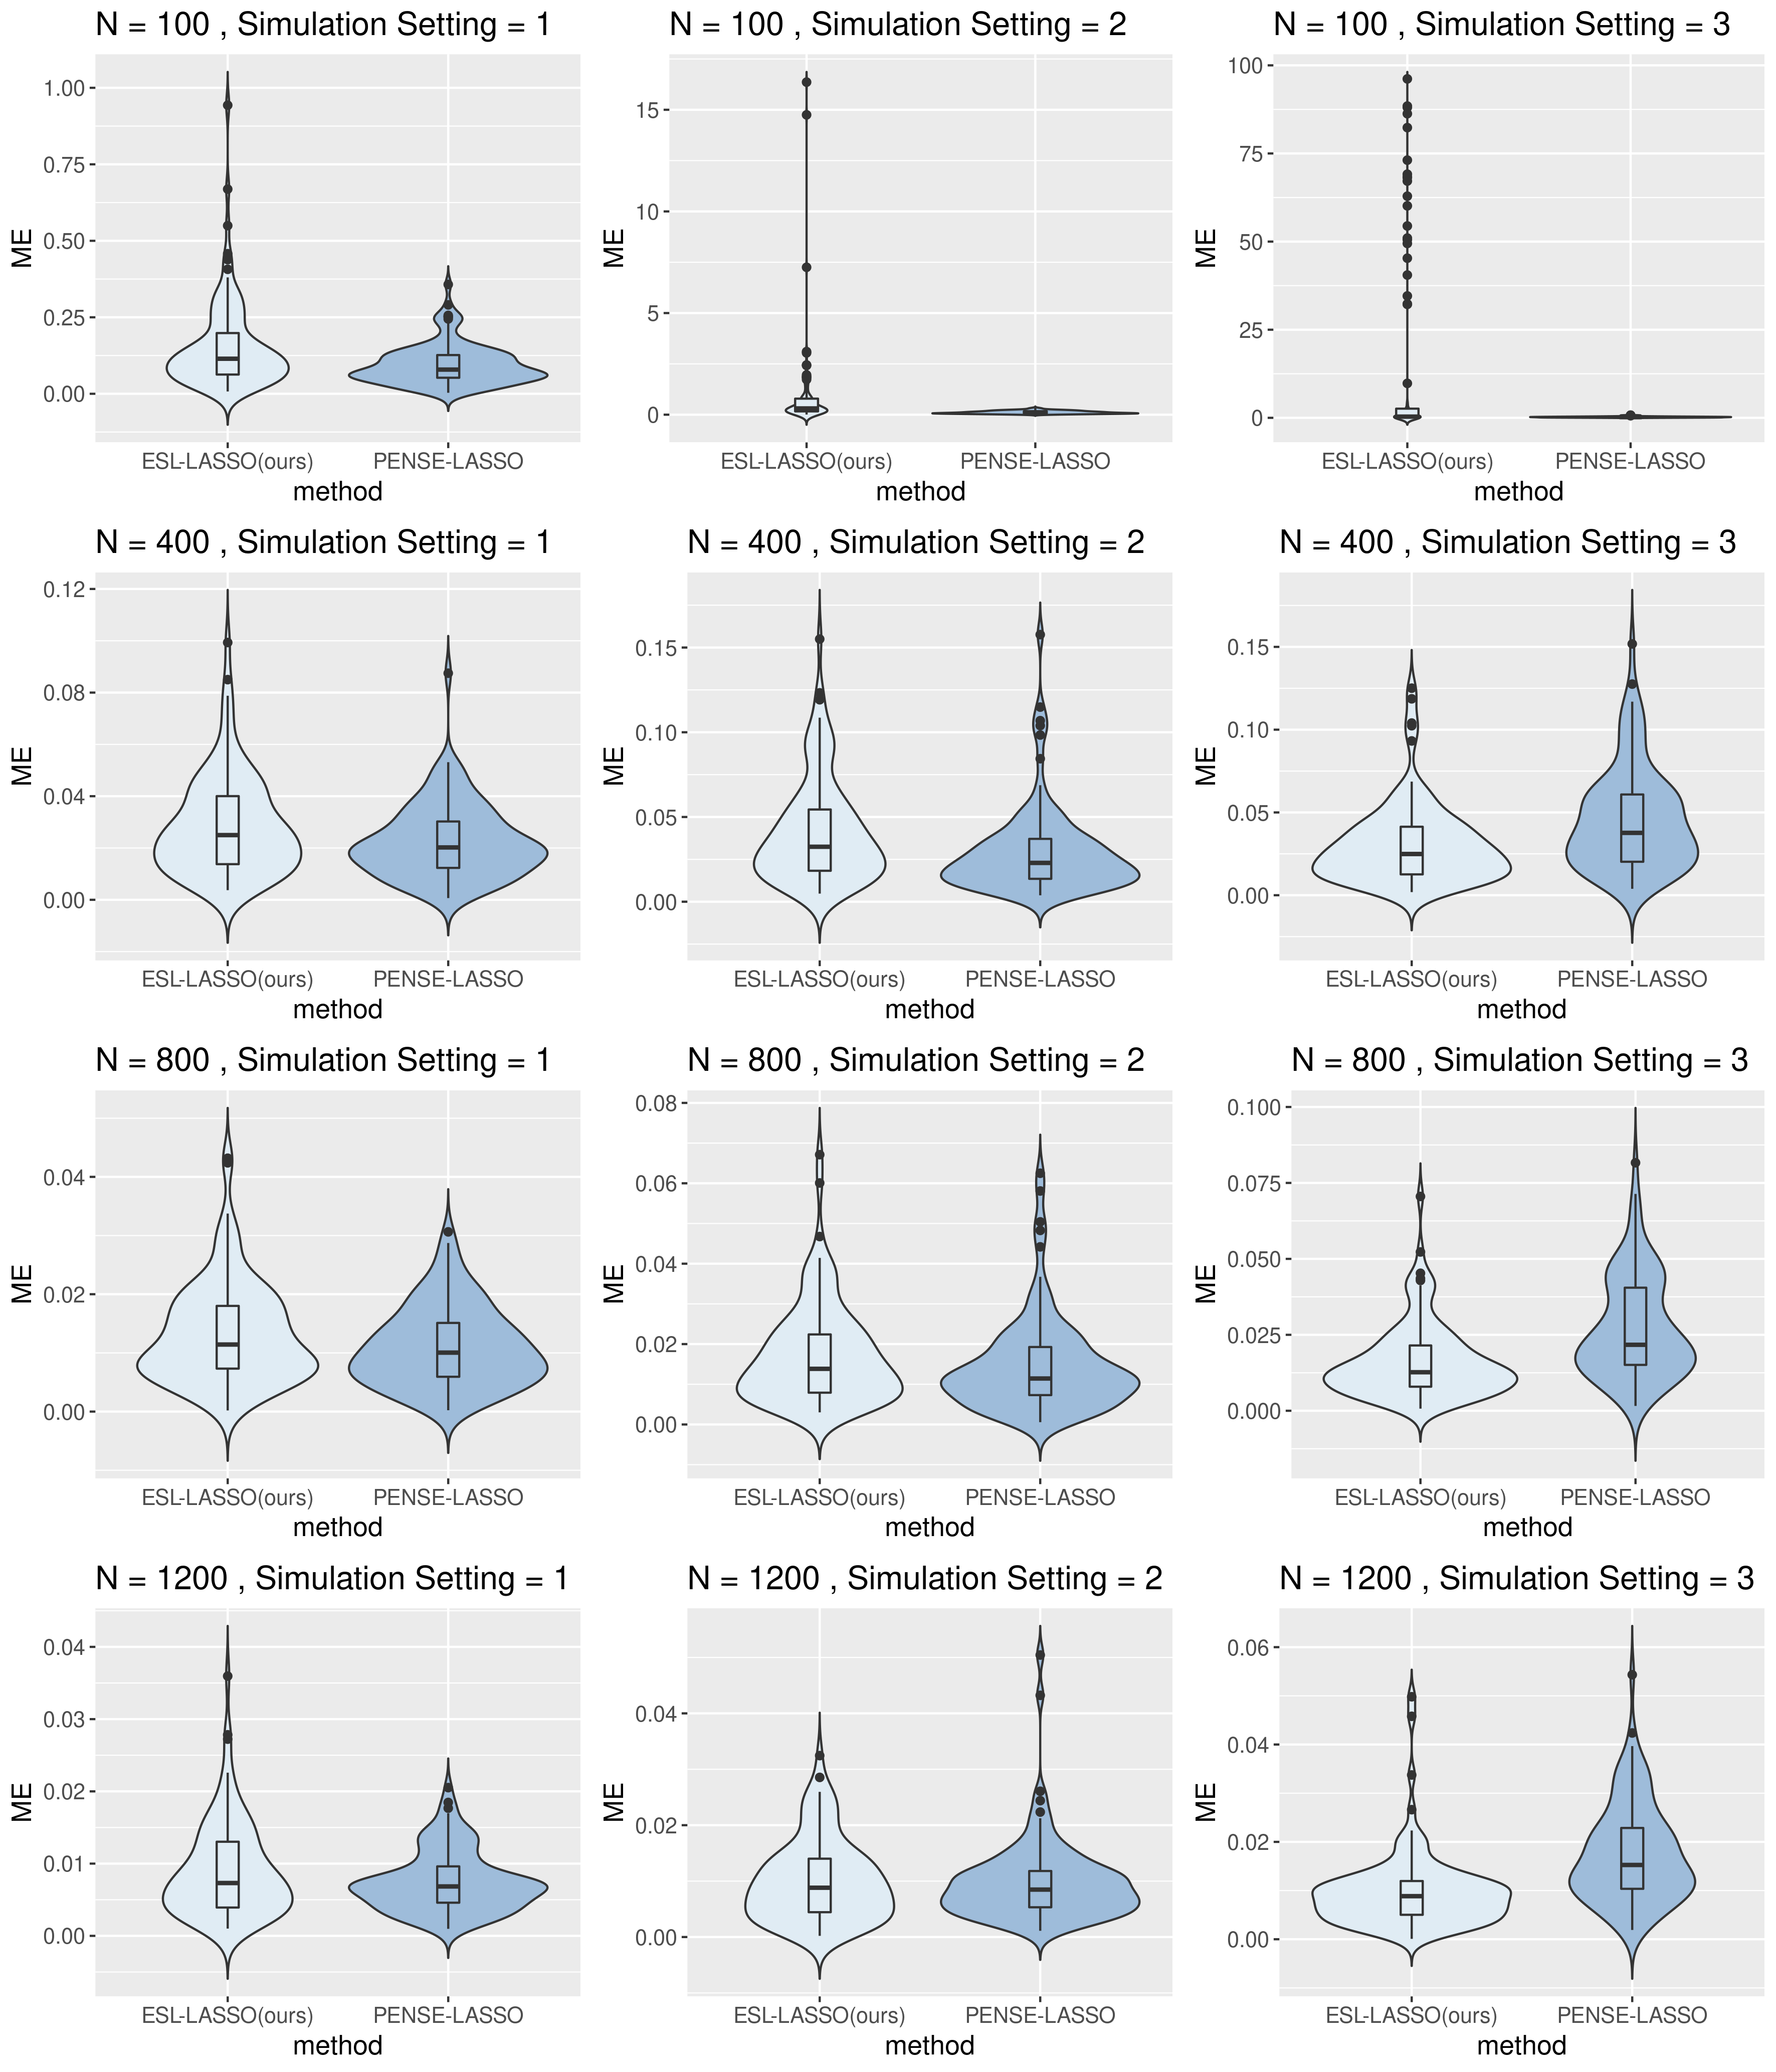
\includegraphics[width = \linewidth]{figures/ME_compare.png}
    \caption{Violin plots for the ME across all simulation settings. For each subfigure, the violin plot places two kernel density vertically with a box plot in the center. }
    \label{fig:me}
\end{figure}


In this section, we compare the quality of our version of ESL-LASSO (\cref{alg:esl_lasso}) with the LASSO version of PENSE \citep{freue2019robust} on three simulation settings that described in the paper. For each setting, we repeat both estimation methods for $100$ trials by generating $100$ datasets. And we test the performance of both methods across different samples sizes, i.e.,  $n = 100, 400, 800, 1200$.  
In general we set $d = 8$ and the true coefficients $\beta = \beta  =(1, 1.5, 2, 1, 0,0,0,0)^T$. 
We consider the following three data generating mechanisms:
\benum
\item Influential points in covariates: for $i = 1, 2, \dots, n$, 
\[
x_i &\distiid 0.8 \distNorm(0, I) + 0.2 \distNorm(3 \ind, \Omega), \quad [\Omega]_{i,j} = 0.5^{|i-j|}\\
\eps_i &\distiid \distNorm(0,1).
\]

\item Influential points in response: for $i = 1, 2, \dots, n$, 
\[
x_i &\distiid \distNorm(0\ind, \Omega), \quad [\Omega]_{i,j} = 0.5^{|i-j|}\\
\eps_i &\distiid 0.8\distNorm(0,1) + 0.2 \distNorm(10, 6^2).
\]

\item Influential points in both covariates and the response: for $i = 1, 2, \dots, n$, 
\[
x_i &\distiid 0.8 \distNorm(0, I) + 0.2 \distNorm(3 \ind, \Omega), \quad [\Omega]_{i,j} = 0.5^{|i-j|}\\
\eps_i &\distiid \distNamed{Cauchy}(0,1)
\]
\eenum


For ESL-LASSO, we repeat the complete procedure twice and base the proximal gradient descent with $50000$ iterations. For PENSE-LASSO, we use four-fold cross-validation to select the penalty constant that leads to the minimal mean square prediction error. In terms of the measure of performance, we evaluate both the variable selection precision---including PSR \citep{chen2008extended} and NSR \citep{fan2001variable}, which measures the proportion of true features selected by the methods and the proportion of discarded features with true zero coefficients respectively---and the model error proposed by the author, i.e.,
\[
\text{ME} = (\hat \beta - \beta_0)^T \left( \frac{1}{n} \sum_{i =1}^n x_i x_i^T\right)   (\hat \beta - \beta_0).
\]

As shown in \cref{fig:sr}, as sample size gets larger, ESL-LASSO shows better variable selection precision comparing to PENSE-LASSO, where both PSR and NSR are $1$ for $n =400, 800, 1200$. PENSE-LASSO is able to recover the true variables but have problem with discarding the variables with true zero coefficients. ESL-LASSO may benefit from the adaptive LASSO penalty while PENSE-LASSO uses the LASSO penalty, of which the performance may potentially be improved if we employ the same adaptive LASSO penalty to PENSE.
One may also notice that the performance of ESL-LASSO is not ideal when $n = 100$, such phenomenon is more clearly displayed in \cref{fig:me}, indicating that ESL-LASSO may suffer from numerical instability with small data size. 


Next, \cref{fig:me} gives a quantitative characterization of the relative performance of ESL-LASSO and PENSE-LASSO. As demonstrated in the plot,  in the first two simulation settings, ESL-LASSO displays a similar performance asymptotically as PENSE-LASSO. But in the third setting, where the influential points are introduced in both the covariates and the response,  ESL-LASSO behaves quite bad when $n  =100$ and gets slightly better than PENSE-LASSO as the sample size increases. 












\section{Discussion} \label{sec:dis}

This report provides a comprehensive discussion of the exponential squared loss regression employed with an adaptive LASSO regularizer, with a particular focus on its computational strategy. We point out potential issues in the optimization treatment to the ESL-LASSO objective and propose an efficient algorithm that is able to at least solve the objective function locally, while the original scheme can produce ill-defined results.
We also modified the original tunning constant selection method, making the whole procedure easier to implement and makes the ESL-LASSO more reliable. Also, we are unable to recover the simulation results included in the paper, where our empirical results for the original ESL-LASSO methods is abnormally bad. We suspect that the authors tune the search range of $\gamma$ for the simulation experiments. 


The original paper provides a descent theoretical treatment to the variable
selection process in a robust regression setting and attempts to design the
computation scheme based on these asymptotic results. However, their approach
indicates some fundamental misunderstanding to the robust regression problem.
In general, blindly aiming for the oracle property or optimal efficiency of a
robust estimator is not appropriate as there is usually a trade-off between the
robustness and efficiency. A practical way is to minimize the asymptotic
variance under a bound on the bias \citep[p. ~68]{maronna2019robust}. 

Another important element for robust regression problem is the initial value. Provided that most robust regression problem involves non-convex optimization, the choice of the initial value can significantly affects the final results. \citet{wang2013robust} chooses the MM-estimator as both the initial value and the pilot estimator used in the adaptive LASSO penalty, which prevents the application of this method to a high-dimensional setting where the MM-estimator could return some zero coefficients. To further polish the ESL-LASSO methods, we might want to include some data-driven methods to obtain a better initial value.









%%%%%%%%%%%%%%%%%%%%%%%%%%%%%%%%%%%%%%%%%%%%%%%%%%%%%%%%%%%%%%%%%%%%%%%%%
%% Reference
%%%%%%%%%%%%%%%%%%%%%%%%%%%%%%%%%%%%%%%%%%%%%%%%%%%%%%%%%%%%%%%%%%%%%%%%%%
\newpage
\bibliographystyle{apalike}
\bibliography{sources}


%%%%%%%%%%%%%%%%%%%%%%%%%%%%%%%%%%%%%%%%%%%%%%%%%%%%%%%%%%%%%%%%%%%%%%%%%
%% Appendix
%%%%%%%%%%%%%%%%%%%%%%%%%%%%%%%%%%%%%%%%%%%%%%%%%%%%%%%%%%%%%%%%%%%%%%%%%%
\newpage
\appendix



\end{document}
